\chapter{Testing}

\section{Introduction}

Softawre testing is an integral part of agile software development - with the use of Feature-Driven Development, it is important to know when a feature has reached the state of 'done', and this is typically once automated tests have confirmed that the functionality works as intended. \cite{Karam1} Radigan explains that incorporating agile testing practices, such as those used in FDD or Test-Driven Development (TDD) are a great way of minimising technical debt, and allowing for QA (Quality Assurance) staff to 'keep up with development'. \cite{Radigan1}

The Laravel framework is reportedly built for 'testing in mind', and PHPUnit, a xUnit (akin to JUnit) testing framework for PHP developed by Sebastian Bergmann is included by default. There are also browser-facing testing tools included under Laravel Dusk, but due to time-constraints were omitted. The autokmated tests used by this application were therefore all written in PHPUnit. \cite{Laravel10} \cite{Bergmann1}


\section{Automated Testing}

\begin{figure}[!ht]
    \centering
    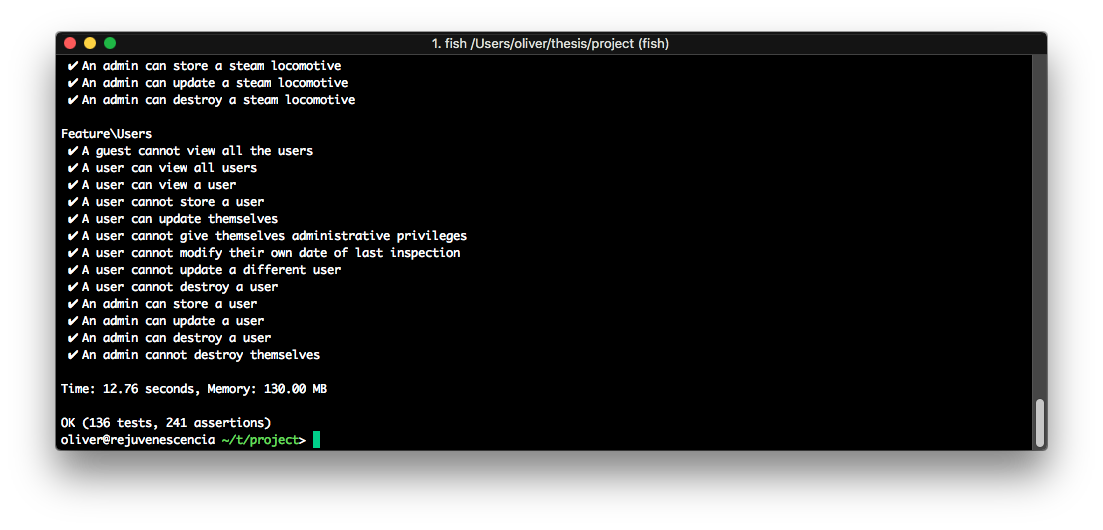
\includegraphics[width=1.0\textwidth]{Figures/tests}
    \caption{Screenshot of PHPUnit running, and successfully running all available tests.}
    \label{fig:testscmd}
\end{figure}

Two subdirectories are defined within the tests directory, one for unit tests, and the other for feature testing. All tests from both subdirectories are executed when PHPUnit is directed to begin testing. Two base classes also exist within this parent directory for subsequent tests to extend from; these files are provided by Laravel. \cite{Laravel10}

A characteristic shared by both types of test is their use of a \texttt{setUp} method, which can set up certain parameters for testing, such as the use of a predefined volunteer user or adminstrator user for testing, so that they do not need to be set up with each test. \texttt{DatabaseMigrations} is also imported into the class to instruct PHPUnit to ensure that database migrations are ran before testing commences, so that tests do not attempt to run on a blank dummy database, and subsequently fail as tables they depend upon, do not exist. \cite{Laravel10}

Finally, all tests are written with method names resembling sentences, with a prefix of 'test'. This is so that when tests are run, as shown in figure \ref{fig:testscmd}, the purpose of each test is parsed into a readable sentence.

\textbf{The full results of unit and feature testing can be found in Appendix \ref{Automated Test Results}.}

\subsection{Unit Testing}
Unit tests are designed to test very specific parts of the application, such as specific methods within classes. According to Hamill, a unit test should 'test a particular behaviour within the production code. Its success or failure validates a single unit of code'. \cite{Hamill1}

An example unit test is this code taken from one of the program's unit test classes:

\begin{lstlisting}[language=PHP, breaklines]
    public function test_an_operation_shift_can_derive_its_parent_operation()
    {
        $this->assertNotNull($this->getShift()->create()->operation);
    }
\end{lstlisting}

The purpose of this test can very quickly be derived from its method name - that it checks whether a shift can derive its parent operation. As nested resources, all shifts must be attached to some resource, and if the associated operation cannot be derived using an Eloquent method (i.e. \texttt{\$shift->operation}) then that shift is likely to be orphaned, or a regression has happened somewhere that has broken the relationship defined between the classes. Unit tests exist to ensure that these regressions are picked up on as immediately as they occur, a concept known as regression testing. \cite{Hopping1}

\subsection{Feature Testing}
In contrast to unit tests, feature tests test complex behaviour that can span across different methods. The approach here is that for each resource, every route is tested for the appropriate response in accordance with expected behaviour, combined with the use of negative testing - to ensure that behaviour that a user should not be able to is accounted for as best as possible. \cite{Fornal1}

\begin{lstlisting}[language=PHP, breaklines]
    public function test_an_admin_can_store_an_operation()
    {
        $this->actingAs($this->admin);
        $operation = factory('App\Operation')->make();

        $response = $this->post(route('operations.store'), $operation->toArray());

        $response->assertRedirect();
        $this->assertDatabaseHas('operations', [
            'is_running' => $operation->is_running,
            'notes' => $operation->notes,
        ]);
    }
\end{lstlisting}

In this test, the entire \textit{operation.store} route is tested to ensure that those with administrative privileges can create new operations. An administrator has already been built by the testing suite, so the \texttt{actingAs} method tells PHPUnit that user will be used to carry out actions and will be authenticated as such. An operation is then generated, and the test attempts to POST this to the route, as would normally happen by a HTML form. The response to this is stored within \texttt{\$response} for assertions to be made against its contents.

PHPUnit is expecting the response to have redirected the user, and then proceeds to check that the database contains the operation that was posted. If this is the case, then we know that this was successful.

The reverse test equivalent to this checks that users cannot attempt to store operations of their own, like thus:

\begin{lstlisting}[language=PHP, breaklines]
    public function test_a_user_cannot_store_an_operation()
    {
        $this->actingAs($this->user);
        $operation = factory('App\Operation')->make();

        $response = $this->post(route('operations.store'), $operation->toArray());

        $response->assertForbidden();
        $this->assertDatabaseMissing('operations', [
            'is_running' => $operation->is_running,
            'description' => $operation->description,
        ]);
    }
\end{lstlisting}

The test works in a near identical way, with the same preliminary actions being taken, except this time a pre-generated user without admin privileges has been used. The assertions however this time, are that instead of being redirected, that the application has returned a HTTP 403 Forbidden error code, and that the entry created has not been saved to the database.

\section{Manual Testing}
Some manual testing was done to complement the automated test coverage, primarily for the authentication routes - being able to log in, log out, register, and reset a password. Though automated testing is used for the vast majority of the application behaviour, manual testing can be complementary for behaviour that is user-focused and not 'black and white' - Nordeen goes on to explain the importance of both in parallel: 'testers must ddispell old black-and-white notions of manual testing versus automation testing. Both have their place in modern sofware development, and it's more a matter of knowing when and where to use each.' \cite{Nordeen1}

Manual testing tables are available on Appendix \ref{Manual Test Results}.

\section{Laravel Telescope}

\begin{figure}[!ht]
    \centering
    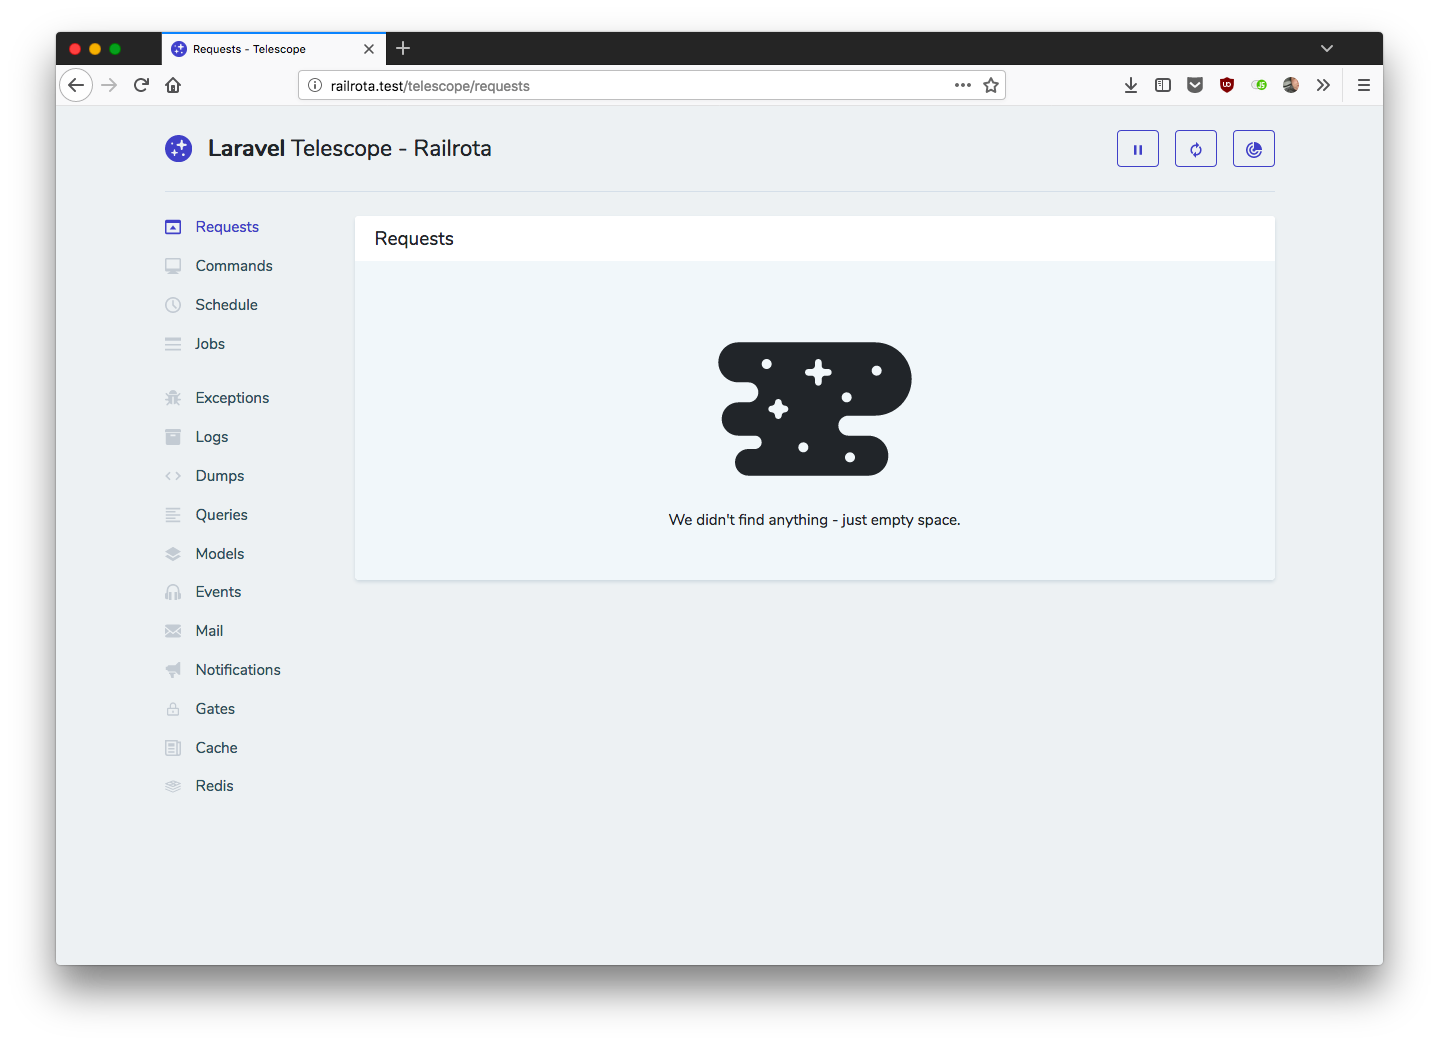
\includegraphics[width=1.0\textwidth]{Figures/screenshot-telescope}
    \caption{Screenshot of the Laravel Telescope interface.}
    \label{fig:telescope}
\end{figure}

Telescope is a debug assistant, that allows authorised users to inspect recent database queries, recent exceptions, log entries, and other useful information for diagnosing problems with the application. This is incredibly useful in the development process, but can be helpful for quickly uncovering problems in production also. \cite{Laravel11} \cite{Abati1}

It is not automatically included or installed with Laravel and must be installed manually. Admin users that are authorised to access Telescope whilst it is running in production mode can be defined by their IDs within the \texttt{.env} environment file.

This functionality was left included as it was immensely useful during the development process to simplify the often tedious and complex process of debugging PHP, and as it is protected by authentication and authorisation, there are no immediate downsides leaving it in the codebase.